\documentclass{article}
\usepackage[utf8]{inputenc}
\usepackage{clrscode3e}
\usepackage[english]{babel}
\usepackage{blindtext}
 \usepackage{graphicx}
 \usepackage{hyperref}
 \hypersetup{
    colorlinks=true,
    linkcolor=blue,
    filecolor=magenta,      
    urlcolor=cyan,
}
\urlstyle{same}
\pagestyle{plain}
\begin{document}

\graphicspath{ {./images/} } 
\begin{titlepage}
 
   \begin{center}
   
       \vspace*{1cm}
       \Huge
       \textbf{Artificial Intelligence Homework} \vspace{1 cm}
       
       \textbf{Archer Problem}
            
       \vspace{1 cm}
      \LARGE
       \textbf{Buzdug\u{a} Ionu\c{t} Gabriel}\\
       Group CEN 2.1B\\
       Year 2\\
       Computer and Information Technology-English
       \vfill
            
      
            
       \vspace{0.8cm}
      
    
    \end{center}
  \end{titlepage}
\newpage

\section {\Large Problem Statement} \vspace*{1cm}
\Large \textbf{Archer arrangement problem} \vspace*{1cm}
\par Let us suppose the k ×k grid presented in Figure 2. The grid is configured with
a pattern of walls. You are required to place n archers on this grid such that
they cannot shoot each other. An archer can shoot up, down, left, right and
also diagonally and its shoot can reach at most w locations in all directions, up
to the grid edges.
\par i)Write a detailed formulation for this search problem.
\par ii)Identify a search algorithm for this task and explain your choice.
\begin{figure}[h]
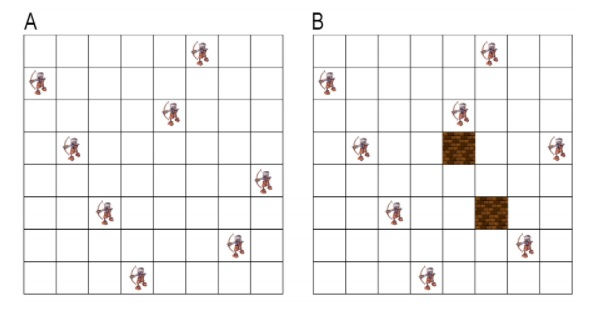
\includegraphics[width=12 cm, height=5cm]{figure2}
\end{figure}
\par Figure 2: Valid arrangements of archers so that they cannot shoot each other.
(A) no walls added. (B) two walls added such that the archer in the last col-
umn cannot shoot the archer in the second or fourth column. Note that these
solutions do not contain any two archers on the same row, column and diagonal
of the grid so they are valid for whatever value of w.
\newpage
\section {\Large Problem Requirements} \vspace*{1cm}
\begin{enumerate}
  \item \textbf{Write a detailed formulation for this search problem.}
  \par In this problem our goal is to manage to fit a number of n archers on
  a grid with the dimensions k xk without them attacking each other.
  \par The solution that I found in order to solve this search problem follows the
  model presented in Chapter 5 of the Artificial Intelligence course.
  \begin{itemize}
  \item States:Any arrangement of 0 to n Archers on the board
  \item Initial state:No Archer on the board.
  \item Succsesor Function:Add an Archer to an empty field on the board.
  \item Goal test:n Archers on the board such that no Archer attacks another
  \item Path Costs:0 (we are only interested in the solution).
\end{itemize}
  \item \textbf{Identify a search algorithm for this task and explain your choice.}
  \par For this task I chose to use the Depth First Search(DFS) algorithm in order to implement the problem.
\end{enumerate}
\newpage
\section {\LARGE Pseudocode}
\Large \par In this section it will be presented the Search Algorithm that I used to solve the problem
\par The Depth first Search Algorithm is used for finding the solutions of arrangements for the archers and walls on the grid.It is a uninformed search strategy.Tha main idea is to use this algorithms because it explores each path possible(each arrangement of the board) until there are no more succesor nodes(no more solutions available).

\subsection{Depth First Tree Search Pseudocode}
\Large
\begin{codebox}

\Procname{$\proc{depth\_first\_tree\_search}(problem,n,R)$}
\li
\While $frontier$\Do\li
  $node \gets frontier.pop()$\li
 \If $problem.goal\_test(node.state) $      \Then \li Print the grid solution \End
 \li $frontier.extend(node.expand(problem))$
\End \End 
\li return None



\end{codebox}
 \vspace*{1cm}
\par With this search algorithm I was able to find multiple arrangements of archers and walls for given the maximum number of archers that we can put on a grid.
\newpage

\newpage
\par Here we can observe how the time complexity behaves in our algorithm.
\par Search Space –  Search space of our problem consists of a total of  $N^{N}$ states, corresponding to all possible configurations of the N Archers on board.
\par Therefore, the worst-case time complexity of our algorithm is O($N^{N}$). But, this worst-case occurs rarely in practice and thus we can safely consider our solution as a optimal one.\vspace*{1cm}
\par This is the graph which shows how the O($N^{N}$) behaves.
\begin{figure}[h]
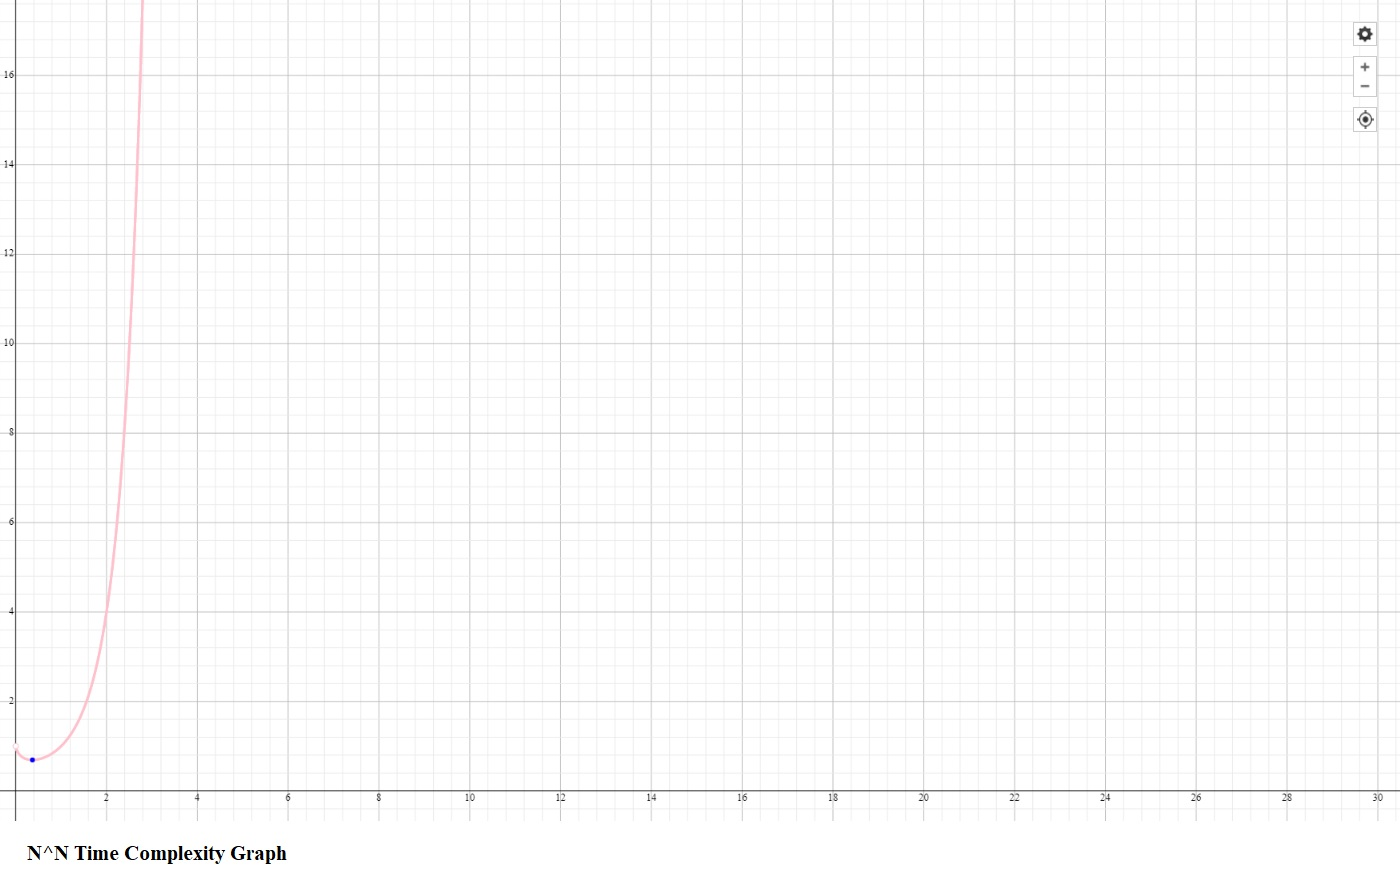
\includegraphics[width=12 cm, height=10cm]{AssignmentReport/images/figure4.jpg}
\end{figure}

\newpage
\section{Application Outline}
\subsection{High Level Application Structure}
\par In this section we review the modular structure of our application on a high level hierarchy. 
\begin{figure}[h]
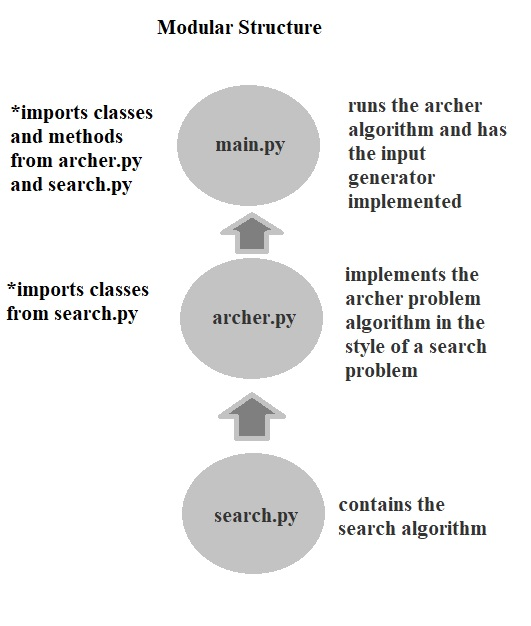
\includegraphics[width=12 cm, height=10cm]{figure3}
\end{figure}
\par Our program uses a modular structure so that it can be easily divided 
in different work files.
\par All the ".py" files are part of the project structure and are interconnected by importing the classes and methods needed between the files as you can see in the above picture.
\newpage
\subsection{Description of input data}
\par Our input data is relevant to what the algorithm needs to work and contains:
 \begin{itemize}
     \item An integer \textbf{N} which represents the number of archers That need to fit on the board.
    \item An integer \textbf{w} which represents the range of the archers.
     \item A list variable named \textbf{restrict} which contains on what positions will the walls that block the archers be placed.
    \item We also got a list variable named \textbf{placement} which initializes the empty board which will be used to place the archers onto.
   \end{itemize}
\subsection{Description of output data/results}
\par In the results section it is presented how the output data sets of the problem
are being made.
\par The output data is consists of:
 \begin{itemize}
     \item The number of walls that will be placed on the grid.
     \item Then for each correct arrangement of archers and walls
     it will be printed the \textbf{pattern} list which holds the position of each archer
     then the position where the walls take place and then a representation of 
     a grid with the archers and the walls placed on it.The program will display arrangements until there are no more solution to be found.
   \end{itemize}
\newpage
\subsection{List of Application modules}
\begin{enumerate}
  \item The search.py module
  \par Here we have implemented the all the neccesary classes and methods for the search algorithm.
  \par The module consists of two classes and two other functions:
  \begin{itemize}
  \item Class \textbf{Problem} (The abstract class for the  formal problem.Which will be subclassed and have it's methods implemented.)
  \item Class \textbf{Node} (Which is a node in a search tree. Contains a pointer to the parent (the node that this is a successor of) and to the actual state for this node.).
  \item Function $\textbf{depth\_first\_tree\_search}$(Searches the deepest nodes in the search tree first.
        Search through the successors of a problem to find a goal.It also acts as our output of data function.)
  \item Function $\textbf{find\_walls}$(which is a function that helps to identify the positions of the walls in the \textbf{restrict} list and is used in the previous function.)
\end{itemize}
  \item The archer.py module:
  \par In this module we have implemented the algorithm for the search problem.
  \par The module consists of one Class:
  \begin{itemize}
  \item Class \textbf{ArcherProblem} (The problem of placing N archers on an k xk grid with none attacking
    each other.)
  
\end{itemize}
  \item The main.py module
  \par This module has two purposes:
  \begin{itemize}
  \item Prepares the input data used for the problem(both manually and random generated)
  \item Runs the algorithm function in order to solve the Archer problem. 
\end{itemize}
\end{enumerate}
\subsection{List of all classes/procedures/functions used in the application}
\par Some of the parameters listed that are not described here,will be described using comments on the source code
\begin{enumerate}
    \item search.py
   \begin{itemize}
       \item Class \textbf{Problem(object)}\\
       The abstract class for a formal problem.
       \par This Class ia used as a template for the methods we need to create the problem algorithms.
       \textbf {Parameters:}
       
       \begin{itemize}
           \item The only  parameter is \textbf{$object$}
           (which is a new style way in python to define a class)
          
           
       \end{itemize}
       \textbf {Methods:}
        \begin{itemize}
           \item  $\_\_init\_\_(self, initial, goal=None):s)$
           (The constructor specifies the initial state, and possibly a goal
        state, if there is a unique goal.)
            \item actions(self, state):(Return the actions that can be executed in the given
        state.)
        \item result(self, state, action):(Return the state that results from executing the given
        action in the given state.)
        \newpage
        \item $goal\_test(self, state):$Return True if the state is a goal. The default method compares the
        state to self.goal or checks for state in self.goal if it is a
        list
        \item $path\_cost(self, c, state1, action, state2):$(Return the cost of a solution path that arrives at state2 from
        state1 via action)
        \item value(self, state):(For optimization problems, each state has a value.)
       \end{itemize}
       \item Class \textbf{Node}\\
       A node in a search tree. Contains a pointer to the parent (the node
    that this is a successor of) and to the actual state for this node.
       \\\textbf{Methods:}
       \begin{itemize}
           \item  $\_\_init\_\_(self, state, parent=None, action=None, path\_cost=0):$
           \\Create a search tree Node, derived from a parent by an action
           \item expand(self, problem):\\List the nodes reachable in one step from this node.
           \item $child\_node(self, problem, action):$
           \\Returns the child of the current node
           
       \end{itemize}
       \item Function $depth\_first\_tree\_search(problem,archerNumber,restrict):$
       \\Searches the deepest nodes in the search tree first.
        Searches through the successors of a problem to find a goal.
        \\This is where we also print our output data for each correct arrangement found by going through each node.
       \item $find\_walls(restrict,archer):$
         \\The parameter restrict is a list and it is used to mark where the walls are going to be placed,while the archer parameter it is used to verify if an Archer on the position archer is on the same position as a wall.
         \\The functions either returns True or False.
   
   \end{itemize} 
  \item archer.py 
  \par This module only contains one Class:
  \begin{itemize}
      \item Class ArcherProblem(Problem):
      \par The problem of placing N Archers on an kxk grid with none attacking
    each other.  A state is represented as an N-element array, where
    a value of r in the c-th entry means there is a queen at column c,
    row r, and a value of -1 means that the c-th column has not been
    filled in yet.  We fill in columns left to right.
    \\The Class only takes one parameter which is the Class Problem(implemented before in search.py)
    \\The Methods of class ArcherProblem are:(the parameters and the return values of each method will be described in the source code as comments)
    \\
    \textbf {Methods:}
        \begin{itemize}
          \item $\_\_init\_\_(self, N,w,placement):$
          \\it always gets called when a new ArcherProblem object is created
          \item actions(self, state):
          \\In the leftmost empty column, try all non-conflicting rows.
          \item result(self, state, row):
          \\Place the next Archer at the given row.
          \item conflicted(self, state, row, col):
          \\Would placing an archer at (row, col) conflict with anything?
          \\this is the first conflicting condition
          \item conflicted1(self, state, row, col):
          \\this is the second conflicting condition
          \item conflict(self, row1, col1, row2, col2):
          \\it is used in the conflicted method
          \\Check if  no conflicts.
          \item conflict1(self, row1, col1, row2, col2):
          \\it is used in the conflicted1 method
          \\Check if  no conflicts.
          \item $goal\_test(self, state):$
          \\Check if all columns filled, no conflicts.
       \end{itemize}
    
  \end{itemize}
  \item main.py
  \\This is the main module that acts as a start up file,imports classes and functions from the other two modules and has the \textbf{input generator} implemented in this way:
  \\k(the size of the grid is randomly generated between 4 and 10 size[because there are too few solutions for k less than 4)
  \\w(the range of archers also gets a random int between 0,k-1)
  \\W(is the number of walls is also randomly generated between 0,k-1)
  \\we construct the restrict list which holds the position of each wall is placed
  
  
  \newpage
 
  
\end{enumerate}
\newpage

\par \textbf{Conclusions}
\par Working on this problem helped me understand more about the course and the importance of search problems.
\par There are multiple new things that I learned while working on this project:
\begin{enumerate}
    \item First of all,it helped me to improve my coding ability by interacting with new types of ways to solve problems.
    \par The Artificial Intelligence approach to solving problems is very interesting because it mimics the human thinking and applies it to our algorithms.
    \par That is because search problems are designed to reach a  goal state by modifying,checking,and keeping count of other states.
    \item Secondly,I believe another key factor that has improved my ability to solve problems is having to make a report about the problem I am working with.
    \par Being able to enunciate a problem in a formal way can undoubtedly improve our knowledge about the problem,but also about programming in general.
    \par The main factors of this are in my opinion The application outline and the experimental data sections.
    \par The first one has a big role in helping how to structure the algorithm in from modules interactions to classes,functions and other similar things.
    \par Meanwhile,the latter helps to verify that our problem works on multiple sets of data and the output data is clearly developed to both me and the reader.
\end{enumerate}
\newpage
\subsection {References}
\begin{enumerate}
\item \href{https://www.geeksforgeeks.org/}{GeeksforGeeks.com}
\item \href{https://stackoverflow.com/}{StackOverflow.com}
\item The chapters and laboratories of the Artificial Intelligence course .

\end{enumerate}
\end{document}


